\section{Evaluation and Discussion}
\label{sec:evaluation}

We conduct a set of experiments to evaluate our approach with different combinations of features and classification techniques. The goodness of classification results is measured by $5$ common metrics, which are precision, recall, accuracy, F1-score and Area under Curve (AUC). All detailed results are shown in Table \ref{tab:data1}. We have trained classifiers with $70\%$ tweets from both sarcastic and normal datasets. Later, we test the classifier with separated dataset which contained the $30\%$ of the dataset.\\

\begin{figure}[hbt]
\centering
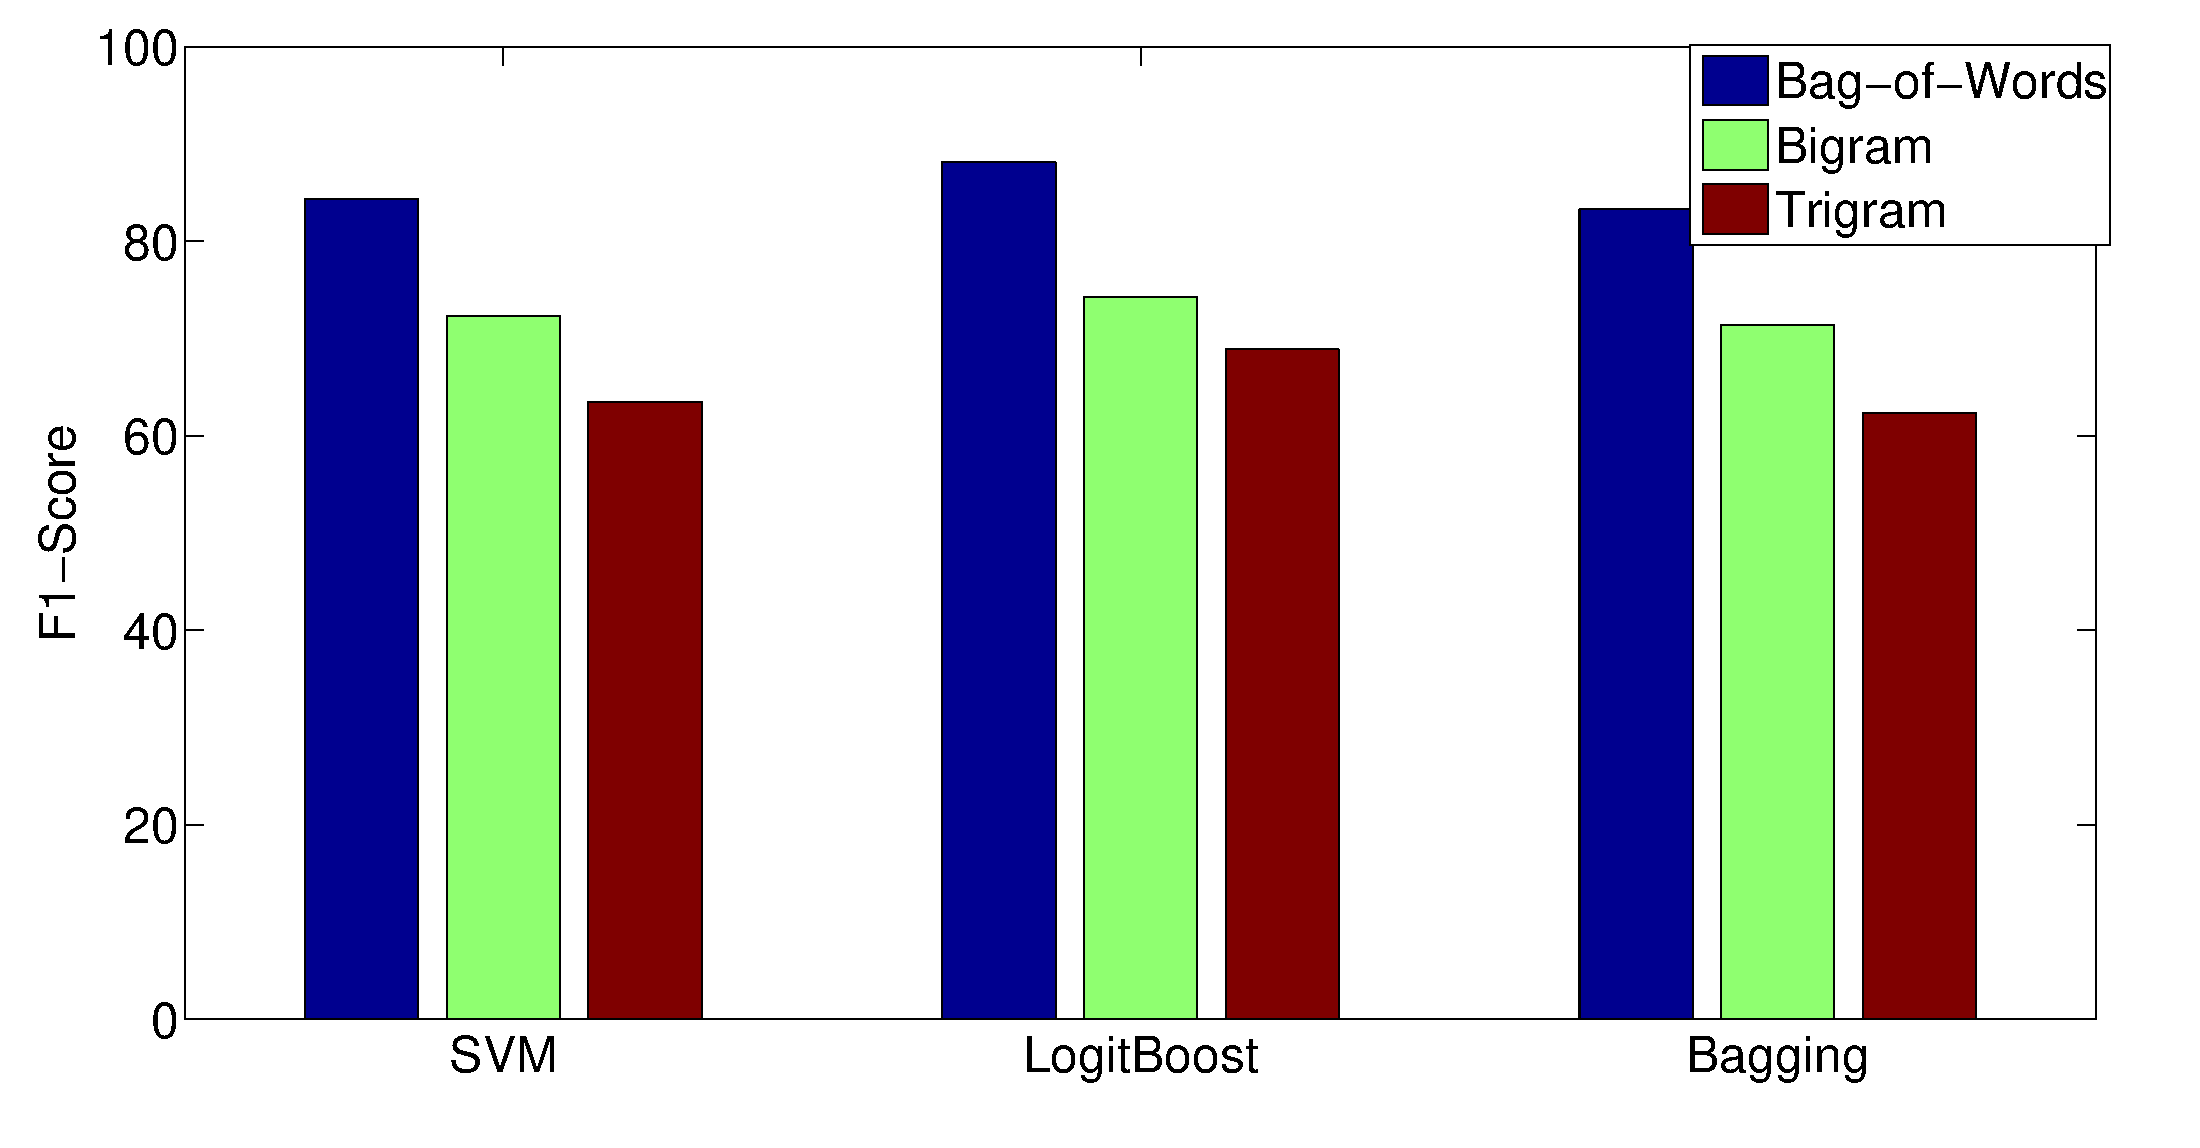
\includegraphics[width=3in, height= 2.4 in]{./figs/bow.eps}
\caption{Effect of different language model specific training in different SSD classifiers}
\label{train:fig}
\end{figure}

Among various features, language models perform the best, and syntactic features result in serious over-fitting. Fig. \ref{train:fig} shows the results when using different language models. The bag-of-words which corresponds to the unigram language model achieves $10\%$ and $19\%$ higher accuracy compared with bigram and trigram, respectively. Due to highly flexible word usage in tweets, bigrams and trigrams are rarely common. However, we can always see some common bag-of-words since sarcastic tweets contain sentiment related words like ``love'', ``hate'', ``favor'', etc. Frequent occurrence of these words can efficiently distinguish sarcastic tweets from normal tweets.\\

From the results, we can see that lexical features and syntactic features are easy to make classifiers overfitted. The reduction of accuracy is around $18\%$ and $22\%$ for lexical features and syntactic features compared with the bag-of-words feature. Unlike normal English sentences, tweets generally contain many punctuation, emoticons, etc. The results for lexical features demonstrate that only considering lexical features can not accurately identify sarcastic tweets. That is, lexical features are not in fact specific to sarcastic tweets. Syntactic features are even worse than lexical features. One possible reason is the words which do not have syntactic function will significantly confuse the construction of syntactic dependency trees. However, we have observed that even though single type of features might fail, but combining them may result in better predictions.\\

Combining social features with all other possible features we can improve the accuracy to a value over $95\%$. The significant improvements demonstrate social features are more efficient to characterize a sarcastic tweet. From our dataset, we found that a large portion of sarcastic tweets have named entities embedded. As long as having recognized named entities, common sentiments towards them make sarcastic tweets more classifiable. Moreover, social strength also helps to identify the likelihood that tweets, fitting other sarcastic features, have similar probabilities to be sarcastic tweets if their social strength are at the same level. Therefore, social features which aim to capture dependencies among tweets are better than lexical features and syntactic features to characterize sarcastic tweets.\\

\begin{figure}[hbt]
\centering
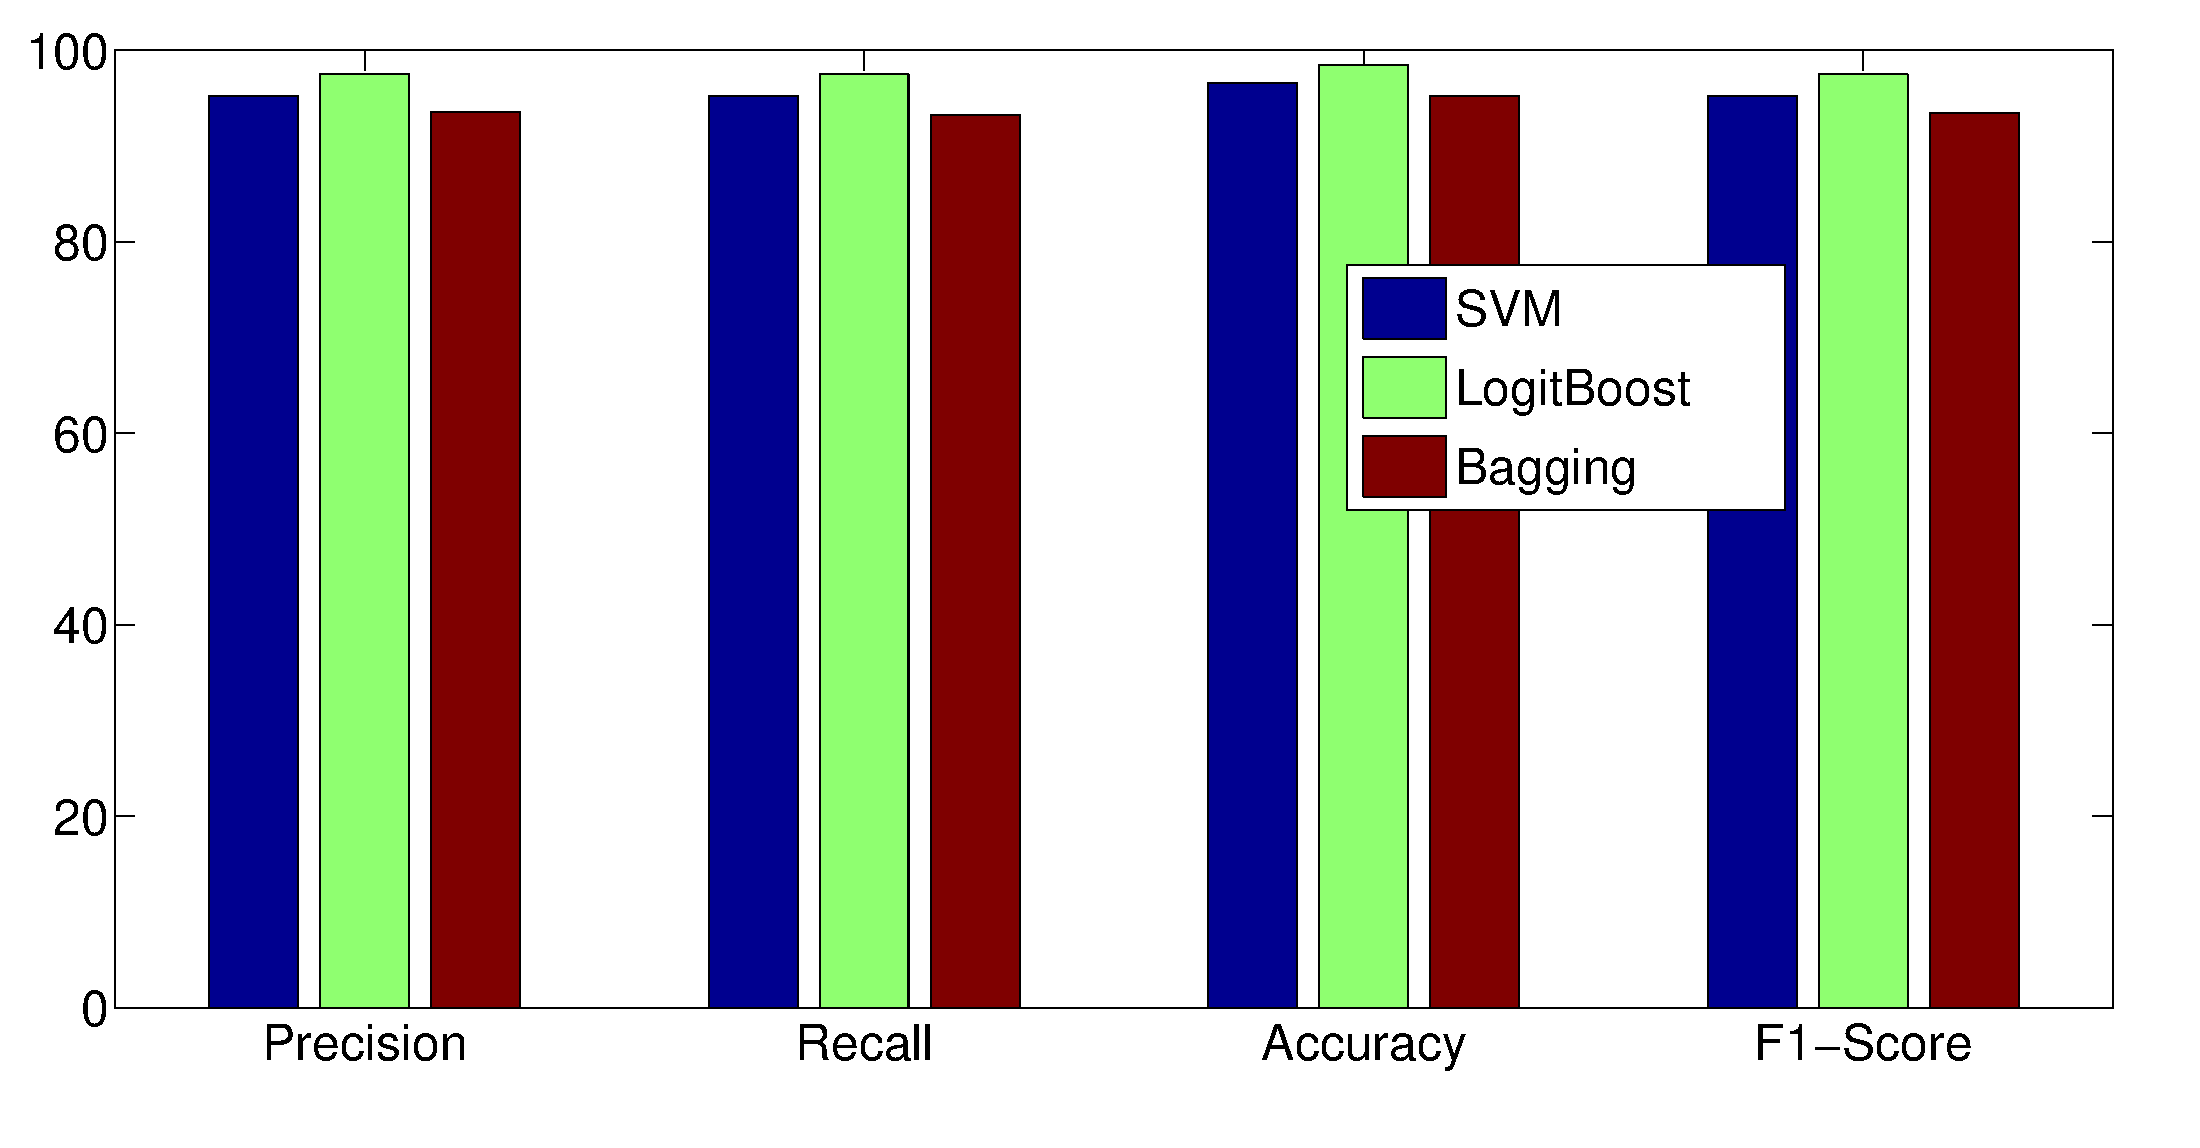
\includegraphics[width=3in, height= 2.4 in]{./figs/class.eps}
\caption{Comparison of Precision, Recall, F1-Score and Accuracy of different SSD classifiers}
\label{fig:classifier}
\end{figure}

Fig. \ref{fig:classifier} demonstrates the results when applying various classifiers with all features we can use. Initally, we have employed SVM classifier with linear kernel for classifying sarcastic tweets, and got reasonable F1-score with realtively less training time. However, later we have also tried with different ensemble techniques like boosting (using Weka implementation) and bagging (using EnsembleSVM implementation) as it is reported to perform better in literature. Although overall performance of LogitBoost with Decision Stump is the best, the gain is not significant.\\

\begin{figure}[hbt]
\centering
\includegraphics[width=3.4in, height= 2.4 in]{./figs/compare_systems.eps}
\caption{Comparison of a few competing techniques with SSD}
\label{fig:comparison}
\end{figure}

We compare our results with other state-of-art approaches in Fig. \ref{fig:comparison} and Table \ref{tab:data2}. SASI \cite{davidov10} uses a semi-supervised approach with mainly pattern based lexical feature whereas authors of \cite{tomas14} used varied set of lexical and semantic features. The performance gain is around $34\%$ compared to \cite{davidov10} mainly due to its pattern based approach which suffers from overfitting. Moreover, around $3\%$ accuracy improvement has been achieved by our proposed approach SSD compared to the method proposed in \cite{tomas14}. Since almost all other possible lexical features and syntactic features have been evaluated by our work and other related work, tweet dependencies characterized by social features are more important than those features to classify sarcastic tweets.

\begin{table*}[htb]
%\renewcommand{\arraystretch}{1.9}
  \centering
  {\small
    %\vspace{-0.1in}
  \begin{tabular}{|@{~}l@{~~}|@{~~}l@{~}|@{~~}l@{~}|@{~~}l@{~}|@{~~}l@{~}|@{~~}l@{~}|@{~~}l@{~}|}
\hline
Feature set & Method used & Precision & Recall & Accuracy & F1-Score & AUC \\\hline
Bag-of-Words & SVM with linear kernel & $84.0475$ & $84.6621$ & $83.6177$ & $84.3674$ & $86.5413$ \\\hline
Word Bigram & SVM with linear kernel & $72.0175$ & $72.3411$ & $73.5127$ & $72.3132$ & $77.1137$  \\\hline
Word Trigram & SVM with linear kernel & $63.8823$ & $63.2914$ & $64.7732$ & $63.4913$  & $67.3412$  \\\hline
Only Lexical Feature & SVM with linear kernel & $62.0813$ & $62.2723$ & $65.1184$ & $62.3213$   & $68.9023$ \\\hline
Only Syntactic Feature & SVM with linear kernel & $58.5623$ & $59.4112$ & $61.5234$ & $58.8232$  & $66.6784$ \\\hline
All Features with Social Features & SVM with linear kernel & $\mathbf{95.2358}$ & $\mathbf{95.2218}$ & $\mathbf{96.6023}$ & $\mathbf{95.2288}$   & $\mathbf{97.7812}$ \\\hline
Bag-of-Words & Logitboost & $88.1239$ & $88.1239$ & $90.0324$ & $88.1239$  & $92.2013$  \\\hline
Word Bigram & Logitboost with Decision Stump & $73.3487$ & $74.2375$ & $76.5123$ & $74.2234$   & $79.7613$ \\\hline
Word Trigram & Logitboost with Decision Stump & $68.8812$ & $68.8812$ & $72.1276$ & $68.8812$   & $74.2314$ \\\hline
Only Lexical Feature & Logitboost with Decision Stump & $64.0823$ & $64.0823$ & $67.4098$ & $64.0823$  & $70.2349$  \\\hline
Only Syntactic Feature & Logitboost with Decision Stump & $60.6756$ & $60.6756$ & $63.5454$ & $60.6756$  & $64.0873$ \\\hline
All Features with Social Features & Logitboost with Decision Stump & $\mathbf{97.4568}$ & $\mathbf{97.4568}$ & $\mathbf{98.4176}$ & $\mathbf{97.4568}$ & $\mathbf{98.8876}$ \\\hline
Bag-of-Words & Bagging with SVM & $83.0475$ & $83.5611$ & $84.5177$ & $83.2674$ & $85.3413$ \\\hline
Word Bigram & Bagging with SVM & $71.2713$ & $71.4531$ & $73.3427$ & $71.3412$  & $75.1745$ \\\hline
Word Trigram & Bagging with SVM & $62.8845$ & $62.2914$ & $68.7732$ & $62.3457$ & $70.3456$ \\\hline
Only Lexical Feature & Bagging with SVM  & $58.0823$ & $58.0127$ & $61.2384$ & $58.0432$  & $63.4523$  \\\hline
Only Syntactic Feature & Bagging with SVM  & $53.1256$ & $53.1256$ & $56.8674$ & $53.1256$  & $59.0234$ \\\hline
All Features with Social Features & Bagging with SVM & $\mathbf{93.5812}$ & $\mathbf{93.1846}$ & $\mathbf{95.1456}$ & $\mathbf{93.3825}$  & $\mathbf{97.3216}$ \\\hline
%\vspace{-0.15in}
\end{tabular}
  }
 \vspace{0.1in}
  \caption{Summary of Results for running SVM, Boosting, and Bagging with different feature sets on datasets.}
%\vspace{-0.25in}
  \label{tab:data1}
\end{table*}

\begin{table}[htb]
%\renewcommand{\arraystretch}{1.9}
  \centering
  {\small
    %\vspace{-0.1in}
  \begin{tabular}{|@{~}l@{~~}|@{~~}l@{~}|@{~~}l@{~}|@{~~}l@{~}|@{~~}l@{~}|}
\hline
Technique & Precision & Recall & F1-Score & Accuracy\\\hline
SASI \cite{davidov10} & $74.27$ & $70.67$ & $72.43$ & $78.68$\\\hline
Coling '14 \cite{tomas14} & $91.23$ & $91.23$ & $91.23$ & $95.77$\\\hline
SSD & $97.46$ & $97.46$ & $97.46$ & $98.89$\\\hline
%\vspace{-0.15in}
\end{tabular}
  }
 \vspace{0.05in}
  \caption{Comparing different supervised techniques of Sarcasm Detection in Twitter with SSD}
%\vspace{-0.25in}
  \label{tab:data2}
\end{table}

% \begin{table}[htb]
% %\renewcommand{\arraystretch}{1.9}
%   \centering
%   {\small
%     %\vspace{-0.1in}
%   \begin{tabular}{|@{~}l@{~~}|@{~~}l@{~}|@{~~}l@{~}|@{~~}l@{~}|@{~~}l@{~}|}
% \hline
% Technique & Precision & Recall & F1-Score & Accuracy\\\hline
% SASI (CoNLL 2010) & $50.67$ & $48.27$ & $49.44$ & $52.68$\\\hline
% Coling 2014 & $53.23$ & $53.23$ & $53.23$ & $59.77$\\\hline
% SSD & $65.46$ & $65.46$ & $65.46$ & $68.89$\\\hline
% %\vspace{-0.15in}
% \end{tabular}
%   }
%  \vspace{0.05in}
%   \caption{Comparing different techniques Sarcasm Detection in Twitter in Czech Dataset}
% %\vspace{-0.25in}
%   \label{tab:data2}
% \end{table}